%%%%%%%%%%%%%%%%%%%%%%%%%%%%%%%%%%%%%%%%%%%%%%%%%%%%
% This will help you in writing your homebook
% Remember that the character % is a comment in latex
%
% chapter 4
\chapter{Decode Stage}
\label{DecodeUnit}

In this part of the datapath the instruction that was previously fetched is broken down and given to several components.
This part of the datapath contains more circuitry with respect to the fetch unit:

\begin{enumerate}
    \item Sign Extender Module and 4to1 multiplexer;
    \item Register File;
    \item Pipe Registers for subsequent execution phase;
    \end{enumerate}

\section {Sign Extender Module and four to one multiplexer}

    The sign extender module is designed with the final goal of interpreting correctly the immidate bit field stored in an immidiate type or jump type instructions.
    In fact, as the implemented DLX gives the possibility to distingush operations for unsigned and signed operations, this combinational block 
    gives the possibility to extend the most significant bit of the immediate field of the immediate type instruction (sixteenth least significant bit) to the the other sixteen bits. 
    The same is done does  for the immediate field of the Jump-Type instructions (this time containing a twentysix bit width instead of sixteen).
    The reason for this choice is because the DLX wires all have thirtytwo bit width, hence we must extend the original immidiate value of the instruction accodingly.
    Furthermore, there are four possible possibilities of interest that could be presented: 
    \begin{enumerate}

        \item an Immidiate-Type instruction interpreting the immediate field as signed: in this case depending on the Most significant bit of the immediate
        bit field, the sixteen additional most signinfiant bits will be either zero, or one. in this scenario we are extending a sixteen bit immediate to a thritytwo bit value
        
        \item an Immidiate-Type instruction interpreting the immediate field as unsigned: in this case regardless of the Most significant bit of the immediate
        bit field, the sixteen additional most signinfiant bits will be zero. in this scenario we are extending a sixteen bit immediate to a thritytwo bit value
     
        \item a Jump-type instruction interpreting the immediate field as as signed: in this case depending on the Most significant bit of the immediate
        bit field, the six additional most signinfiant bits will be either zero, or one. in this scenario we are extending a twenty six bit immediate to a thritytwo bit value

        \item a Jump-type instruction interpreting the immediate field as unsigned: This scenario is not implemented in the datapth as the jump instructions always consider
        a signed value of the immediate field. However for a future improvement of the DLX it could be used for a type of jump instruction that can only jump forward.

        \end{enumerate}

    All these scenarios are performed in parallel in the decode unit, and thanks to a four to one multiplexer, the correct specific scenario is selected for obtaining
    the appropriate extension. Furthermore, the selection bits of the multplexer individuating the correct extension scenario come from two control bits from the control unit.

\section {Register file}

    The Register file of the DLX consists of thirtytwo registers. The register at address zero is always zero by convetion while the thirtysecond
    register is only utlized for the storing of the return address when executing a jal instruction. A main schematic block is shown in Figure 4.2.

\begin{figure}[h!]
    \centering
    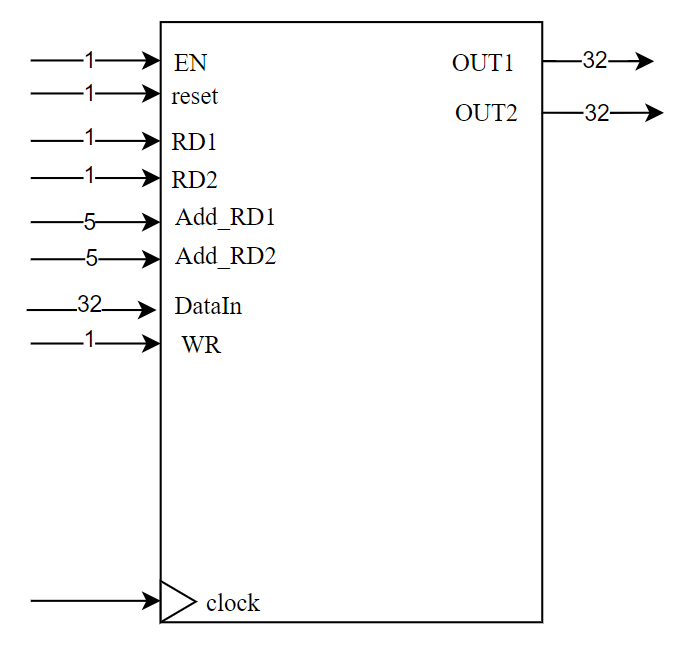
\includegraphics[scale = 0.45]
    {chapters/figures/RegisterFile}
    \caption{Figure 4.2 Register File Schematic }
    \label{fig:RFpic}
    \end{figure}

        \subsection{Reading Methodology}
        The register file has two read ports. The reading is done asynchronously this way it is easier for the register file to obtain the proper
        addresses of the register for which the reading is performed. On the basis of the RD1 and RD2 single bit port signals, the ports for reading can be activated.
        After receiving the proper addresses from the Instruction register bits, the Values of the registers are made available at the OUT1 and OUT2 ports respectively.

        \subsection{Writing Methodology}
        The writing methodology is synchrnous to falling edges of the clock cycle. This is done to avoid the issue of metastability.

        In fact if the register file were to sample the DataIn port at the rising edge of the clock cycle, since the control unit sets the write port
        at rising edges of the clock cycle, the register file would understand as if the write port bit is zero hence leading to an incurrect behavior. Forthermore, 
        this is the reason why the write process is sensitive to the falling edge od the clock.
        About the reset, it is sensistive to the falling edge of the clock and when it is active high. At the start up of the processor, thanks to the reset all the
        registers of the register file as set to inital value zero.

\section {Decode Pipe Registers}

    There are many Pipeline registers which store relative information all of them having syncronous enabling and resetting at the rising edge of the clock cycle:

    \begin{enumerate}

        \item NPC1: This pipeline register is needed as it needs to be propagated to the Execution unit in case there is the need to compute an address 
        because the instruction of interest is a branch or a jump.
        \item RegisterA and RegisterB: These registers store the output of what was read from the asynchronous reading of the register file. If in the decode
        stage there is a Register type instruction both of these registers will be filled with useful values to be later used in execute
        \item ImmREG : This register stores the final extended form of the immediate that was chosed from the four to 1 multiplexer described earlier in this section.
        \item RT and RD Registers: the need of this register is important do the fact that there is a variation  in position of the destination register field of an instruction;
        in fact for immediate type instruction the destination register address is stored in bit field range [20 downto 16]. While for the Register type instruction it is located
        in the bit range [15 downto 11] of the instruction. Hence in the decode both information are stored, to then decide based on the instruciton type which is the correct address
        for writing back to the register file.
        \item IR1: This will keep the instruction that was analyzed during the decode stage also in execute. This register was implemented for viewing the waveforms
        while debugging the processor's course of actions.



        \end{enumerate}
    